\chapter{NewSkillz Behaviour Framework}
\label{chap:rl}

\section{Introduction}
The work presented here describes the new behaviours framework for rUNSWift and is the combined effort of the following authors: Beth Crane, Jack Murray, Dan Padilha, Stephen Sherratt, and Alexander Whillas.

The \textit{NewSkillz} behaviour framework is a new implementation of the \verb!Python!-based control logic for the rUNSWift codebase. The new framework aims to replace the existing \verb!Python! skills by allowing for a much easier learning curve, easily understandable code, the removal of redundancy through abstraction, and less need for complex state transition models. Furthermore, the framework is abstracted in such a way that allows the same behaviour code to be run on the robots as well as in simulators with no modification required.

The 2012 behaviours were ported in a mostly-working state to the \textit{NewSkillz} framework, as a proof-of-concept. Examples in this section will stem from this proof-of-concept implementation.

As it required the effort of many authors, information about \textit{NewSkillz} is spread throughout various reports. In particular, more information about the integration with a simulator and the reasoning behind the framework can be found in the report by Crane and Sherratt.\cite{simulator} The focus of this section therefore is to provide a gentle introduction to implementing skills using the \textit{NewSkillz} framework, as well as documentation of its major features. Note that the terms \textit{behaviour}, \textit{skill}, and sometimes \textit{state}, are used interchangeably throughout the text.

\section{Theory}

The behaviours framework is what controls the behaviour of the Nao robots when playing soccer. Specifically, this refers to all high-level decisions the robots must make. That is to say, the behaviours do \textit{not} define how a robot's body moves in order to make it walk, how the robot analyses a video image to find the ball, or how a robot communicates with its team-mates.

Instead, the behaviours framework defines how a robot decides whether to go for the ball or move to another position, whether to kick the ball or line itself up at a better angle, whether to dive for the ball as a goalie, and so on. This high-level decision-making requires rapid development during the competition in order to adapt to the opposing team strategies. For this reason, a high-level programming language (\verb!Python!) is used for the greatest ease of development.

The \textit{NewSkillz} framework differs from the 2012 skills framework in that it is not programmed explicitly as state-machines. Instead, the states arise from inherent properties of the framework while still being as simple to reason about. State is chosen through a tree-like structure of skills where each skill decides whether to \textit{delegate} its decision to another skill, or to perform some action in a \textit{tick}.

The skill tree can therefore be thought as a form of decision tree or state-machine. Each node in the tree is expected to delegate a decision down to a node below it. Leaf nodes -- those which do not wish to delegate -- are required to therefore perform some sort of action in the real world, such as kick the ball.

To better illustrate this concept, the skill tree for the proof-of-concept port of the 2012 skills is shown in Figure~\ref{fig:skill_tree}.

\begin{figure}[h]
\centering
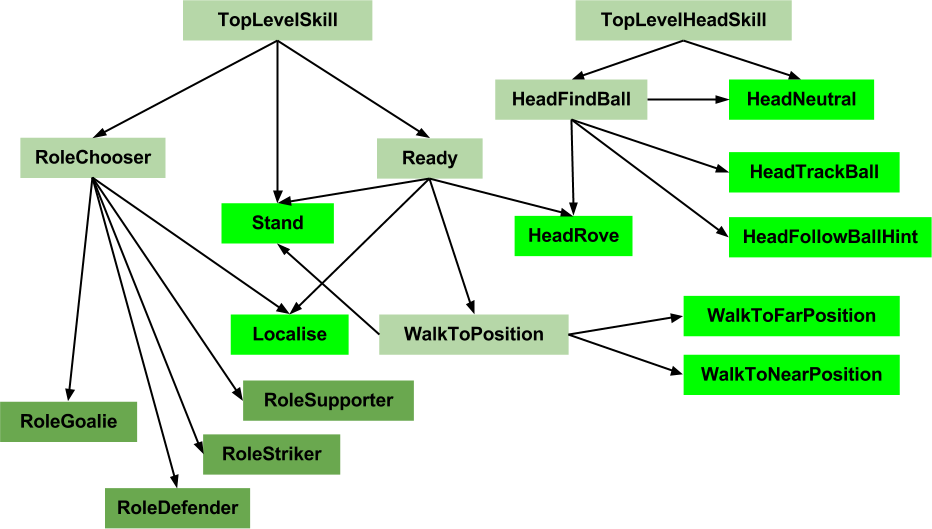
\includegraphics[width=0.9\textwidth]{img/skill_tree.png}
\caption{Tree of the proof-of-concept port of the 2012 skills. Skills in bright green are leaf skills (which must perform some action). Skills in dark green are un-expanded nodes (i.e. the skills they delegate to are not shown). An arrow from a skill represents a delegation to another skill.}
\label{fig:skill_tree}
\end{figure}

Notice that the tree contains two root nodes, being \texttt{TopLevelSkill} and \texttt{TopLevelHeadSkill}. This allows for decisions to be made for the body and head separately.

The skill tree system provides cleaner and less redundant code through the delegation mechanism. It is easy to imagine this by taking the state machine of the head as in the example provided by Figure~\ref{fig:state_machine}.

\begin{figure}[h]
\centering
\begin{subfigure}{0.45\textwidth}
  \centering
  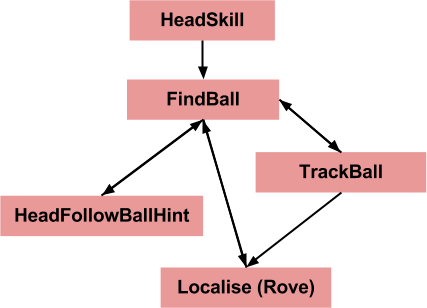
\includegraphics[width=\textwidth]{img/state_machine_old.png}
  \caption{2012 framework}
  \label{fig:state_machine_old}
\end{subfigure}
\begin{subfigure}{0.45\textwidth}
  \centering
  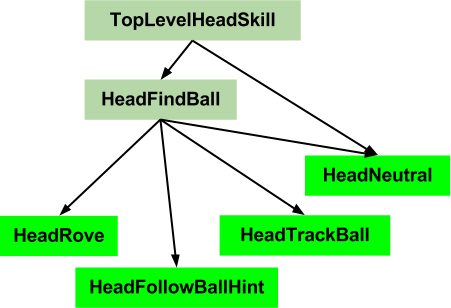
\includegraphics[width=\textwidth]{img/state_machine_newskillz.png}
  \caption{\textit{NewSkillz} framework}
  \label{fig:state_machine_newskillz}
\end{subfigure}
\caption{Example of the state machine approach of the 2012 skills framework, and the \textit{NewSkillz} skill tree approach.}
\label{fig:state_machine}
\end{figure}

While the 2012 state machine may look simpler, code inspection reveals a much more complex system. For starters, each skill (which we will refer to as a state) in the 2012 framework must include a state transition function defining when to transition to a different state. States can transition to states which transition back to the parent states, or they can transition in only one-way -- this requires redundant checks for the condition to transition back into a state. Furthermore, any state can potentially cause an action or only perform state transitions. While this framework allows for much flexibility, it requires a much greater learning curve and unintuitive coding style.

By contrast, the \textit{NewSkillz} skill tree may look equally complicated, but becomes significantly easier to understand and write for once the required properties are understood:

\begin{itemize}
\item All state transitions are one-way.
\item A state/skill may only transition to another state, or perform an action, but not do both.
\end{itemize}

These properties inherently create a state-machine, so they allow for the same flexibility as the 2012 framework, albeit not in the same way. For example, a \textit{NewSkillz} skill cannot possibly be written in such a way that it can do both state transitions \textit{and} perform an action. Instead, the programmer is forced to partition the skill into a decision and its possible actions, leading to simpler modular code.

\section{Implementation}

\subsection{Codebase}

The rUNSWift codebase is split into the \verb!C++! backend and the \verb!Python! behaviours framework. The behaviours framework is run through the \texttt{Perception} thread (running at $30Hz$) in 

\texttt{runswift/robot/behaviour/python/PythonSkill.cpp}

This defines the \verb!C++! to \verb!Python! interface. It also ensures that \textbf{live-reload} for skills works -- a robot can be left running in a crashed state, modified skills can be pushed to it, and it will simply continue running as if it had never crashed.

The \verb!Python! entry-point is located in \texttt{runswift/image/home/nao/data/behaviours/cpp\_glue.py}

On every tick, \texttt{cpp\_glue} ticks both the \texttt{TopLevelSkill} and \texttt{TopLevelHeadSkill}. Because the body's \texttt{TopLevelSkill} is ticked \textit{after} the head, any skills in the body skill tree can choose to delegate to a skill in the head tree and thus \textbf{override} the head tree's actions.

All skills are located in \texttt{runswift/image/home/nao/data/behaviours/skills}

\subsection{In Real Life (IRL)}

The \texttt{IRL} class is an abstraction of the state of the robot, and also an interface to perform actions, such as moving the head, walking, or kicking the ball.

The \texttt{IRL} abstraction works to such that skills can rely on the state (known as \texttt{Sense}) and \texttt{Action}s, regardless of whether they come from the rUNSWift codebase, or from the simulator.\cite{simulator} This clearly allows for the same skills to be used for both platforms, with only the \texttt{Sense}s and \texttt{Actions} being written separately.

\subsubsection{Sense}

The \texttt{Sense IRL} defines a set of functions which provide the state of the robot at any instant. Running on the robots, the \texttt{Sense IRL} works simply as a wrapper for the rUNSWift \texttt{Blackboard}, which provides a shared state between all threads. Examples of \texttt{Sense}s include: \texttt{is\_ball\_visible()}, \texttt{game\_state()}, \texttt{is\_lost()}, and so on.

\texttt{Sense}s are defined in \texttt{runswift/image/home/nao/data/behaviours/robot\_sense.py}

Any skill can access the \texttt{Sense} functions by simply calling \texttt{self.irl.sense.\textit{some\_sense\_function()}}.

\subsubsection{Action}

The \texttt{Action IRL} defines a set of functions for interacting with the 

Any leaf skill can perform an action by calling \texttt{self.irl.action.\textit{some\_action(argument)}}. By definition, actions are only allowed to occur inside the \texttt{tick} function of a skill (see Section~\ref{sec:tick}).

\subsection{Skills}

The \texttt{Skill} class is the ``bread and butter'' of the \textit{NewSkillz} framework. This class abstracts away state transitions entirely from the programmer and provides the \texttt{IRL} to all skills automatically. The class also defines the argument-passing interface for skills.

Every skill in the skill tree is a subclass of \texttt{Skill}. \texttt{Skill} provides two functions: \texttt{tick} and \texttt{delegate}. When implementing a skill, exactly \textbf{one} of these functions must be overloaded, depending on whether the skill expects to \textit{delegate} its decision to another skill, or \textit{tick} an \texttt{IRL} Action.

Both the \texttt{tick} and \texttt{delegate} functions can be defined with required and optional arguments. These arguments are supplied when skills delegate to other skills. This process is described more in Section~\ref{sec:delegate}.

\subsubsection{Tick}
\label{sec:tick}

The \texttt{tick} function is defined only for leaf skills which do not expect to delegate to any other skills, and instead expect to perform some \texttt{IRL} Action.

Good design is to have very atomic leaf skills that perform a single action, perhaps with some parameters, but with little to no conditional logic.

\subsubsection{Delegate}
\label{sec:delegate}

The \texttt{delegate} function is defined only for skills which expect to delegate to another skill to perform some action. These skills perform all the logical decisions about states.

Good design should ensure that skills cannot possibly delegate in a cyclic manner (i.e. traversing the skills tree should guarantee arrival at a leaf skill).

\subsection{Geometry}

A simple geometry library is implemented which defines some \texttt{Vector}-like objects and all associated functions.

The geometry library is in \texttt{runswift/image/home/nao/data/behaviours/geometry.py}

There is one primitive class defined in geometry known as a \texttt{Point}. A \texttt{Point} simply represents an $(x, y)$ tuple. Three subclasses are defined: \texttt{Vector}, \texttt{UnitVector}, and \texttt{DirectionVector}. All of these perform in exactly the same way, and differ only by their initialisations:

\begin{description}
\item[Point] takes an $x$ and $y$ coordinate.
\item[Vector] takes a length and a direction in radians.
\item[UnitVector] takes a direction in radians and becomes a vector of length $1$.
\item[DirectionVector] takes a direction in either degrees or radians and becomes a unit vector.
\end{description}

These geometry classes should be used for any representations of points on the field, direction facing, point to walk to, relative distances, and so on. The \texttt{Point} superclass defines many useful vector functions, including rotations, lengths, subtractions, etc.

An example works as such: if a robot is located at a $robot\_pos = Point(x, y)$, is facing in the $robot\_facing = DirectionVector(45\degree)$, and wants to turn towards the ball at $ball\_pos = Point(x, y)$, then the amount the robot needs to turn is given by the angle:

\begin{equation}
(robot\_pos \gg ball\_pos).rotate(robot\_facing).angle()
\end{equation}

Here, the $\gg$ (right-shift) operator returns the vector from $robot\_pos$ to $ball\_pos$. This vector is then rotated such that the $robot\_facing$ vector becomes the $x-$axis. This gives the vector to the ball relative to the robot's facing direction. Finally, one can extract the angle which the robot needs to rotate to in order to face the ball.

The geometry library thus allows for much simpler calculations to be made for many vector operations.

\subsection{Debugging} 

All \verb!Python! runtime exceptions and errors are caught by \texttt{cpp\_glue}. \texttt{cpp\_glue} keeps watch on the skill-tree in order to print debug information about it, and catches all \verb!Python! exceptions in order to place the robot into ``Emergency mode''.

Under ``Emergency mode'', the robot stops all movement, flashes all its LEDs in random colours, and audibly requests to be picked up (for use in the competition). The stack trace produced by \verb!Python! is able to show the faulting skill as well as its parent skill (which delegated to it), but no further up the line. If a bigger stack trace is required, simply print out the skill name in the \texttt{tick} function of \texttt{Skill}.

Also, thanks to the live-reload functionality built into \texttt{cpp\_glue}, new skills can be pushed to the robot or even edited directly on the robot. Once a \verb!Python! file is modified on the robot, \textit{NewSkillz} reloads all skills and the robot continues from whatever state it was in (as the \texttt{Blackboard} state is preserved).

\section{Results \& Evaluation}

A major advantage resulting from the \textit{NewSkillz} framework is the significant cut down in redundant code due to the abstraction of the \texttt{Blackboard} into the \texttt{IRL} API. By design, all skills have access to the \texttt{IRL}, and therefore to the \texttt{Blackboard} -- which needed to be passed around to everything in the 2012 framework. The standard \texttt{Skill} class also helps to abstract state transitions away, leaving much cleaner code.

\section{Future Work}

% TODO Tick locking
% TODO ncurses
% TODO Port the 2013 competition code

\section{Conclusion}
